% Sección 4: preprocesamiento e ingeniería de características (Rol 1, P2).
% Se inserta con % Sección 4: preprocesamiento e ingeniería de características (Rol 1, P2).
% Se inserta con % Sección 4: preprocesamiento e ingeniería de características (Rol 1, P2).
% Se inserta con % Sección 4: preprocesamiento e ingeniería de características (Rol 1, P2).
% Se inserta con \input{seccion_4_preprocesamiento}. Requiere booktabs.
% Figura: figures/14_particiones_cronologicas.pdf (scripts/03_figura_particiones.py).
% Las cifras provienen de data/processed/*.csv (scripts/01 y 02).

\section{Preprocesamiento e ingeniería de características}
\label{sec:preproc}

\subsection{Conjunto supervisado y variable objetivo}

Cada ejemplo corresponde a un instante $t$ en que se hace el pronóstico. La respuesta es $y_t=\mathrm{PM}_{2{,}5}(t+1)$, la concentración exactamente una hora después, y las entradas usan únicamente mediciones en $t$ o antes. Como la rejilla horaria se conserva completa, el desplazamiento corresponde siempre a una hora real y no al siguiente registro disponible. El valor actual $\mathrm{PM}_{2{,}5}(t)$ es además el pronóstico del baseline de persistencia, por lo que se incluye como entrada.

\subsection{Variables de entrada}

La Tabla~\ref{tab:vars} resume las 11 variables. Los rezagos de 1, 3 y 6 horas capturan la dependencia inmediata observada en la autocorrelación parcial; los de 12 y 24 horas recogen el ciclo diario; y las medias móviles de 3, 6 y 24 horas, que incluyen el instante $t$, resumen el nivel reciente con menor ruido que un valor aislado. Todas se calculan con desplazamientos hacia atrás o ventanas finales, de modo que ninguna contiene información posterior a $t$. Las medias móviles exigen la ventana completa; con un hueco, la fila se descarta.

\begin{table}[t]
\centering
\caption{Variables del conjunto supervisado.}
\label{tab:vars}
\small
\begin{tabular}{@{}p{3.45cm}p{3.95cm}@{}}
\toprule
Variable & Definición \\
\midrule
\texttt{pm25\_t} & $\mathrm{PM}_{2{,}5}(t)$ \\
\texttt{pm25\_lag$k$} & $\mathrm{PM}_{2{,}5}(t-k)$, $k\in\{1,3,6,12,24\}$ h \\
\texttt{pm25\_media$w$h} & media de las últimas $w\in\{3,6,24\}$ h, incluida $t$ \\
\texttt{hora\_objetivo} & hora del día de $t+1$ (0--23) \\
\texttt{dia\_semana\_objetivo} & día de la semana de $t+1$ (0 = lunes) \\
\midrule
\texttt{y\_pm25\_t1} & respuesta: $\mathrm{PM}_{2{,}5}(t+1)$ \\
\bottomrule
\end{tabular}
\end{table}

La hora y el día corresponden a $t+1$, el instante que se pronostica, que se conoce de antemano. Se codifican dentro del pipeline: la hora con seno y coseno, para que las 23:00 y las 00:00 resulten vecinas, y el día de la semana con variables indicadoras, porque el efecto de fin de semana no sigue una senoide. El conjunto sin calendario usa solo las nueve variables de historial, con los mismos ejemplos, lo que permite comparar ambos enfoques en igualdad de condiciones.

\subsection{Faltantes y ventanas incompletas}

No se imputan valores, ni con ceros ni por interpolación. Un instante es utilizable solo si tiene la respuesta y todo su historial; en caso contrario se descarta. De los 20.424 instantes de la rejilla quedan 18.276 (89,5~\%) (Tabla~\ref{tab:perdida}). Los descartes se deben a que 1.034 instantes no tienen respuesta, 1.033 no tienen medición actual, 1.967 tienen algún rezago faltante y 2.060 una media móvil incompleta (las causas se solapan). Como las interrupciones son largas, un solo hueco invalida muchas filas vecinas. Todos los modelos y el baseline se evalúan sobre estas mismas filas, para que las comparaciones no dependan de diferencias de muestra.

\begin{table}[t]
\centering
\caption{Filas descartadas por faltantes (las causas pueden coincidir).}
\label{tab:perdida}
\small
\begin{tabular}{@{}lrr@{}}
\toprule
Concepto & Filas & \% rejilla \\
\midrule
Instantes $t$ en la rejilla & 20.424 & 100,0 \\
Sin respuesta $\mathrm{PM}_{2{,}5}(t+1)$ & 1.034 & 5,1 \\
Sin medición actual & 1.033 & 5,1 \\
Algún rezago faltante & 1.967 & 9,6 \\
Alguna media móvil incompleta & 2.060 & 10,1 \\
\midrule
\textbf{Filas utilizables} & \textbf{18.276} & \textbf{89,5} \\
\bottomrule
\end{tabular}
\end{table}

\subsection{Partición cronológica}

Los datos se dividen en tres bloques contiguos y disjuntos, sin barajar filas: entrenamiento (enero de 2022 a junio de 2023), validación (julio a diciembre de 2023) y prueba (enero a abril de 2024). La partición se asigna según el instante de la respuesta $t+1$, de modo que ninguna etiqueta de entrenamiento cae en el periodo de validación ni una de validación en el de prueba. Una fila de validación sí puede usar como entrada observaciones del periodo de entrenamiento, algo legítimo porque son pasadas. Los cortes se fijaron antes de ver resultados de ningún modelo. El ajuste de hiperparámetros se hará con validación de origen móvil dentro del entrenamiento, nunca con particiones aleatorias.

\begin{table}[t]
\centering
\caption{Conjunto supervisado por bloque (respuesta en \textmu g/m\textsuperscript{3}).}
\label{tab:part}
\small
\begin{tabular}{@{}lrrrrr@{}}
\toprule
Bloque & Filas & Media & Mediana & P95 & Máx. \\
\midrule
Entrenamiento & 11.551 & 32,9 & 27,8 & 72,2 & 191,5 \\
Validación & 4.024 & 25,1 & 23,7 & 41,8 & 125,3 \\
Prueba & 2.701 & 17,8 & 16,1 & 32,2 & 101,9 \\
\bottomrule
\end{tabular}
\end{table}

La Tabla~\ref{tab:part} y la Fig.~\ref{fig:part} muestran que la distribución de la respuesta cambia entre bloques: la media baja de 32,9 a 17,8 y el máximo de 191,5 a 101,9. El modelo se entrena, por tanto, en un régimen de concentraciones más altas del que se evalúa. Esto obliga a reportar las métricas por bloque y a comparar cada modelo con la persistencia calculada sobre el mismo bloque, ya que un mismo error absoluto no significa el mismo desempeño relativo en cada tramo.

\begin{figure}[t]
\centering
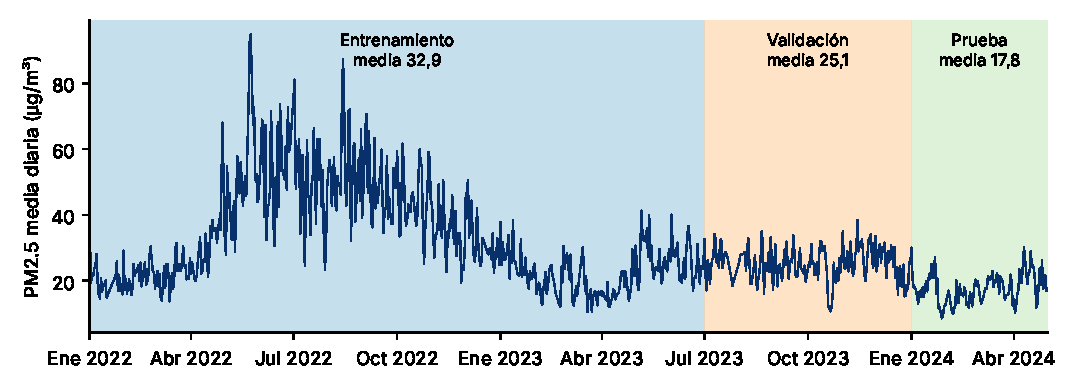
\includegraphics[width=\columnwidth]{figures/14_particiones_cronologicas.pdf}
\caption{Partición cronológica sobre la media diaria de PM2.5 (días con al menos 18 horas medidas). Se indica la media de la respuesta de cada bloque.}
\label{fig:part}
\end{figure}

\subsection{Preprocesamiento dentro del pipeline y prevención de fuga}

El escalado se ejecuta dentro de un \texttt{Pipeline} de scikit-learn: las nueve variables de historial se estandarizan con la media y la desviación del entrenamiento, y esos parámetros se aplican sin reajuste a validación y prueba. Ajustar el escalador con todos los datos filtraría información de los bloques posteriores: la media de $\mathrm{PM}_{2{,}5}(t)$ es de 32,94 en entrenamiento y de 28,98 en el conjunto completo.

La ausencia de fuga se comprueba de forma explícita con un guion reproducible (\texttt{scripts/02\_verificar\_fuga.py}) que ejecuta 12 verificaciones, todas superadas (Tabla~\ref{tab:fuga}). La prueba central altera por completo los valores posteriores a un instante de corte y comprueba que las entradas en ese instante no cambian. Como control negativo, se añade a propósito una variable con información futura y se confirma que la prueba la detecta.

\begin{table}[t]
\centering
\caption{Comprobaciones de ausencia de fuga de información.}
\label{tab:fuga}
\small
\begin{tabular}{@{}p{5.9cm}c@{}}
\toprule
Comprobación & Resultado \\
\midrule
Recálculo independiente con solo el pasado (500 filas) & Superada \\
Las entradas no cambian si se altera el futuro (8 cortes) & Superada \\
Respuesta igual a $\mathrm{PM}_{2{,}5}(t+1)$ y calendario de $t+1$ & Superada \\
Bloques ordenados, disjuntos y completos & Superada \\
Filas con hueco excluidas, sin ceros inventados & Superada \\
Escalador ajustado solo con entrenamiento (con y sin calendario) & Superada \\
Control negativo: una fuga deliberada es detectada & Superada \\
\bottomrule
\end{tabular}
\end{table}
. Requiere booktabs.
% Figura: figures/14_particiones_cronologicas.pdf (scripts/03_figura_particiones.py).
% Las cifras provienen de data/processed/*.csv (scripts/01 y 02).

\section{Preprocesamiento e ingeniería de características}
\label{sec:preproc}

\subsection{Conjunto supervisado y variable objetivo}

Cada ejemplo corresponde a un instante $t$ en que se hace el pronóstico. La respuesta es $y_t=\mathrm{PM}_{2{,}5}(t+1)$, la concentración exactamente una hora después, y las entradas usan únicamente mediciones en $t$ o antes. Como la rejilla horaria se conserva completa, el desplazamiento corresponde siempre a una hora real y no al siguiente registro disponible. El valor actual $\mathrm{PM}_{2{,}5}(t)$ es además el pronóstico del baseline de persistencia, por lo que se incluye como entrada.

\subsection{Variables de entrada}

La Tabla~\ref{tab:vars} resume las 11 variables. Los rezagos de 1, 3 y 6 horas capturan la dependencia inmediata observada en la autocorrelación parcial; los de 12 y 24 horas recogen el ciclo diario; y las medias móviles de 3, 6 y 24 horas, que incluyen el instante $t$, resumen el nivel reciente con menor ruido que un valor aislado. Todas se calculan con desplazamientos hacia atrás o ventanas finales, de modo que ninguna contiene información posterior a $t$. Las medias móviles exigen la ventana completa; con un hueco, la fila se descarta.

\begin{table}[t]
\centering
\caption{Variables del conjunto supervisado.}
\label{tab:vars}
\small
\begin{tabular}{@{}p{3.45cm}p{3.95cm}@{}}
\toprule
Variable & Definición \\
\midrule
\texttt{pm25\_t} & $\mathrm{PM}_{2{,}5}(t)$ \\
\texttt{pm25\_lag$k$} & $\mathrm{PM}_{2{,}5}(t-k)$, $k\in\{1,3,6,12,24\}$ h \\
\texttt{pm25\_media$w$h} & media de las últimas $w\in\{3,6,24\}$ h, incluida $t$ \\
\texttt{hora\_objetivo} & hora del día de $t+1$ (0--23) \\
\texttt{dia\_semana\_objetivo} & día de la semana de $t+1$ (0 = lunes) \\
\midrule
\texttt{y\_pm25\_t1} & respuesta: $\mathrm{PM}_{2{,}5}(t+1)$ \\
\bottomrule
\end{tabular}
\end{table}

La hora y el día corresponden a $t+1$, el instante que se pronostica, que se conoce de antemano. Se codifican dentro del pipeline: la hora con seno y coseno, para que las 23:00 y las 00:00 resulten vecinas, y el día de la semana con variables indicadoras, porque el efecto de fin de semana no sigue una senoide. El conjunto sin calendario usa solo las nueve variables de historial, con los mismos ejemplos, lo que permite comparar ambos enfoques en igualdad de condiciones.

\subsection{Faltantes y ventanas incompletas}

No se imputan valores, ni con ceros ni por interpolación. Un instante es utilizable solo si tiene la respuesta y todo su historial; en caso contrario se descarta. De los 20.424 instantes de la rejilla quedan 18.276 (89,5~\%) (Tabla~\ref{tab:perdida}). Los descartes se deben a que 1.034 instantes no tienen respuesta, 1.033 no tienen medición actual, 1.967 tienen algún rezago faltante y 2.060 una media móvil incompleta (las causas se solapan). Como las interrupciones son largas, un solo hueco invalida muchas filas vecinas. Todos los modelos y el baseline se evalúan sobre estas mismas filas, para que las comparaciones no dependan de diferencias de muestra.

\begin{table}[t]
\centering
\caption{Filas descartadas por faltantes (las causas pueden coincidir).}
\label{tab:perdida}
\small
\begin{tabular}{@{}lrr@{}}
\toprule
Concepto & Filas & \% rejilla \\
\midrule
Instantes $t$ en la rejilla & 20.424 & 100,0 \\
Sin respuesta $\mathrm{PM}_{2{,}5}(t+1)$ & 1.034 & 5,1 \\
Sin medición actual & 1.033 & 5,1 \\
Algún rezago faltante & 1.967 & 9,6 \\
Alguna media móvil incompleta & 2.060 & 10,1 \\
\midrule
\textbf{Filas utilizables} & \textbf{18.276} & \textbf{89,5} \\
\bottomrule
\end{tabular}
\end{table}

\subsection{Partición cronológica}

Los datos se dividen en tres bloques contiguos y disjuntos, sin barajar filas: entrenamiento (enero de 2022 a junio de 2023), validación (julio a diciembre de 2023) y prueba (enero a abril de 2024). La partición se asigna según el instante de la respuesta $t+1$, de modo que ninguna etiqueta de entrenamiento cae en el periodo de validación ni una de validación en el de prueba. Una fila de validación sí puede usar como entrada observaciones del periodo de entrenamiento, algo legítimo porque son pasadas. Los cortes se fijaron antes de ver resultados de ningún modelo. El ajuste de hiperparámetros se hará con validación de origen móvil dentro del entrenamiento, nunca con particiones aleatorias.

\begin{table}[t]
\centering
\caption{Conjunto supervisado por bloque (respuesta en \textmu g/m\textsuperscript{3}).}
\label{tab:part}
\small
\begin{tabular}{@{}lrrrrr@{}}
\toprule
Bloque & Filas & Media & Mediana & P95 & Máx. \\
\midrule
Entrenamiento & 11.551 & 32,9 & 27,8 & 72,2 & 191,5 \\
Validación & 4.024 & 25,1 & 23,7 & 41,8 & 125,3 \\
Prueba & 2.701 & 17,8 & 16,1 & 32,2 & 101,9 \\
\bottomrule
\end{tabular}
\end{table}

La Tabla~\ref{tab:part} y la Fig.~\ref{fig:part} muestran que la distribución de la respuesta cambia entre bloques: la media baja de 32,9 a 17,8 y el máximo de 191,5 a 101,9. El modelo se entrena, por tanto, en un régimen de concentraciones más altas del que se evalúa. Esto obliga a reportar las métricas por bloque y a comparar cada modelo con la persistencia calculada sobre el mismo bloque, ya que un mismo error absoluto no significa el mismo desempeño relativo en cada tramo.

\begin{figure}[t]
\centering
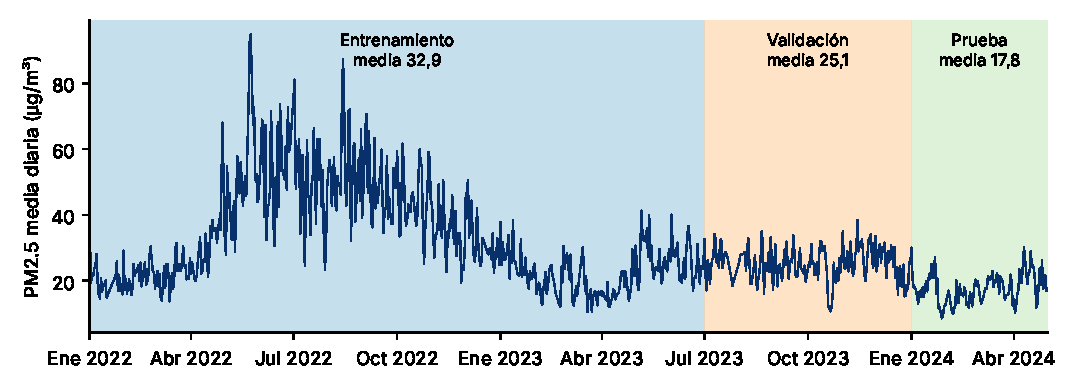
\includegraphics[width=\columnwidth]{figures/14_particiones_cronologicas.pdf}
\caption{Partición cronológica sobre la media diaria de PM2.5 (días con al menos 18 horas medidas). Se indica la media de la respuesta de cada bloque.}
\label{fig:part}
\end{figure}

\subsection{Preprocesamiento dentro del pipeline y prevención de fuga}

El escalado se ejecuta dentro de un \texttt{Pipeline} de scikit-learn: las nueve variables de historial se estandarizan con la media y la desviación del entrenamiento, y esos parámetros se aplican sin reajuste a validación y prueba. Ajustar el escalador con todos los datos filtraría información de los bloques posteriores: la media de $\mathrm{PM}_{2{,}5}(t)$ es de 32,94 en entrenamiento y de 28,98 en el conjunto completo.

La ausencia de fuga se comprueba de forma explícita con un guion reproducible (\texttt{scripts/02\_verificar\_fuga.py}) que ejecuta 12 verificaciones, todas superadas (Tabla~\ref{tab:fuga}). La prueba central altera por completo los valores posteriores a un instante de corte y comprueba que las entradas en ese instante no cambian. Como control negativo, se añade a propósito una variable con información futura y se confirma que la prueba la detecta.

\begin{table}[t]
\centering
\caption{Comprobaciones de ausencia de fuga de información.}
\label{tab:fuga}
\small
\begin{tabular}{@{}p{5.9cm}c@{}}
\toprule
Comprobación & Resultado \\
\midrule
Recálculo independiente con solo el pasado (500 filas) & Superada \\
Las entradas no cambian si se altera el futuro (8 cortes) & Superada \\
Respuesta igual a $\mathrm{PM}_{2{,}5}(t+1)$ y calendario de $t+1$ & Superada \\
Bloques ordenados, disjuntos y completos & Superada \\
Filas con hueco excluidas, sin ceros inventados & Superada \\
Escalador ajustado solo con entrenamiento (con y sin calendario) & Superada \\
Control negativo: una fuga deliberada es detectada & Superada \\
\bottomrule
\end{tabular}
\end{table}
. Requiere booktabs.
% Figura: figures/14_particiones_cronologicas.pdf (scripts/03_figura_particiones.py).
% Las cifras provienen de data/processed/*.csv (scripts/01 y 02).

\section{Preprocesamiento e ingeniería de características}
\label{sec:preproc}

\subsection{Conjunto supervisado y variable objetivo}

Cada ejemplo corresponde a un instante $t$ en que se hace el pronóstico. La respuesta es $y_t=\mathrm{PM}_{2{,}5}(t+1)$, la concentración exactamente una hora después, y las entradas usan únicamente mediciones en $t$ o antes. Como la rejilla horaria se conserva completa, el desplazamiento corresponde siempre a una hora real y no al siguiente registro disponible. El valor actual $\mathrm{PM}_{2{,}5}(t)$ es además el pronóstico del baseline de persistencia, por lo que se incluye como entrada.

\subsection{Variables de entrada}

La Tabla~\ref{tab:vars} resume las 11 variables. Los rezagos de 1, 3 y 6 horas capturan la dependencia inmediata observada en la autocorrelación parcial; los de 12 y 24 horas recogen el ciclo diario; y las medias móviles de 3, 6 y 24 horas, que incluyen el instante $t$, resumen el nivel reciente con menor ruido que un valor aislado. Todas se calculan con desplazamientos hacia atrás o ventanas finales, de modo que ninguna contiene información posterior a $t$. Las medias móviles exigen la ventana completa; con un hueco, la fila se descarta.

\begin{table}[t]
\centering
\caption{Variables del conjunto supervisado.}
\label{tab:vars}
\small
\begin{tabular}{@{}p{3.45cm}p{3.95cm}@{}}
\toprule
Variable & Definición \\
\midrule
\texttt{pm25\_t} & $\mathrm{PM}_{2{,}5}(t)$ \\
\texttt{pm25\_lag$k$} & $\mathrm{PM}_{2{,}5}(t-k)$, $k\in\{1,3,6,12,24\}$ h \\
\texttt{pm25\_media$w$h} & media de las últimas $w\in\{3,6,24\}$ h, incluida $t$ \\
\texttt{hora\_objetivo} & hora del día de $t+1$ (0--23) \\
\texttt{dia\_semana\_objetivo} & día de la semana de $t+1$ (0 = lunes) \\
\midrule
\texttt{y\_pm25\_t1} & respuesta: $\mathrm{PM}_{2{,}5}(t+1)$ \\
\bottomrule
\end{tabular}
\end{table}

La hora y el día corresponden a $t+1$, el instante que se pronostica, que se conoce de antemano. Se codifican dentro del pipeline: la hora con seno y coseno, para que las 23:00 y las 00:00 resulten vecinas, y el día de la semana con variables indicadoras, porque el efecto de fin de semana no sigue una senoide. El conjunto sin calendario usa solo las nueve variables de historial, con los mismos ejemplos, lo que permite comparar ambos enfoques en igualdad de condiciones.

\subsection{Faltantes y ventanas incompletas}

No se imputan valores, ni con ceros ni por interpolación. Un instante es utilizable solo si tiene la respuesta y todo su historial; en caso contrario se descarta. De los 20.424 instantes de la rejilla quedan 18.276 (89,5~\%) (Tabla~\ref{tab:perdida}). Los descartes se deben a que 1.034 instantes no tienen respuesta, 1.033 no tienen medición actual, 1.967 tienen algún rezago faltante y 2.060 una media móvil incompleta (las causas se solapan). Como las interrupciones son largas, un solo hueco invalida muchas filas vecinas. Todos los modelos y el baseline se evalúan sobre estas mismas filas, para que las comparaciones no dependan de diferencias de muestra.

\begin{table}[t]
\centering
\caption{Filas descartadas por faltantes (las causas pueden coincidir).}
\label{tab:perdida}
\small
\begin{tabular}{@{}lrr@{}}
\toprule
Concepto & Filas & \% rejilla \\
\midrule
Instantes $t$ en la rejilla & 20.424 & 100,0 \\
Sin respuesta $\mathrm{PM}_{2{,}5}(t+1)$ & 1.034 & 5,1 \\
Sin medición actual & 1.033 & 5,1 \\
Algún rezago faltante & 1.967 & 9,6 \\
Alguna media móvil incompleta & 2.060 & 10,1 \\
\midrule
\textbf{Filas utilizables} & \textbf{18.276} & \textbf{89,5} \\
\bottomrule
\end{tabular}
\end{table}

\subsection{Partición cronológica}

Los datos se dividen en tres bloques contiguos y disjuntos, sin barajar filas: entrenamiento (enero de 2022 a junio de 2023), validación (julio a diciembre de 2023) y prueba (enero a abril de 2024). La partición se asigna según el instante de la respuesta $t+1$, de modo que ninguna etiqueta de entrenamiento cae en el periodo de validación ni una de validación en el de prueba. Una fila de validación sí puede usar como entrada observaciones del periodo de entrenamiento, algo legítimo porque son pasadas. Los cortes se fijaron antes de ver resultados de ningún modelo. El ajuste de hiperparámetros se hará con validación de origen móvil dentro del entrenamiento, nunca con particiones aleatorias.

\begin{table}[t]
\centering
\caption{Conjunto supervisado por bloque (respuesta en \textmu g/m\textsuperscript{3}).}
\label{tab:part}
\small
\begin{tabular}{@{}lrrrrr@{}}
\toprule
Bloque & Filas & Media & Mediana & P95 & Máx. \\
\midrule
Entrenamiento & 11.551 & 32,9 & 27,8 & 72,2 & 191,5 \\
Validación & 4.024 & 25,1 & 23,7 & 41,8 & 125,3 \\
Prueba & 2.701 & 17,8 & 16,1 & 32,2 & 101,9 \\
\bottomrule
\end{tabular}
\end{table}

La Tabla~\ref{tab:part} y la Fig.~\ref{fig:part} muestran que la distribución de la respuesta cambia entre bloques: la media baja de 32,9 a 17,8 y el máximo de 191,5 a 101,9. El modelo se entrena, por tanto, en un régimen de concentraciones más altas del que se evalúa. Esto obliga a reportar las métricas por bloque y a comparar cada modelo con la persistencia calculada sobre el mismo bloque, ya que un mismo error absoluto no significa el mismo desempeño relativo en cada tramo.

\begin{figure}[t]
\centering
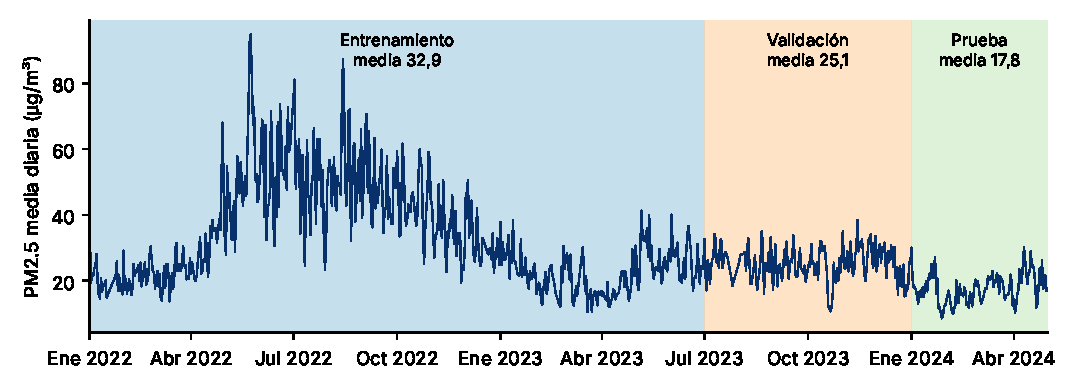
\includegraphics[width=\columnwidth]{figures/14_particiones_cronologicas.pdf}
\caption{Partición cronológica sobre la media diaria de PM2.5 (días con al menos 18 horas medidas). Se indica la media de la respuesta de cada bloque.}
\label{fig:part}
\end{figure}

\subsection{Preprocesamiento dentro del pipeline y prevención de fuga}

El escalado se ejecuta dentro de un \texttt{Pipeline} de scikit-learn: las nueve variables de historial se estandarizan con la media y la desviación del entrenamiento, y esos parámetros se aplican sin reajuste a validación y prueba. Ajustar el escalador con todos los datos filtraría información de los bloques posteriores: la media de $\mathrm{PM}_{2{,}5}(t)$ es de 32,94 en entrenamiento y de 28,98 en el conjunto completo.

La ausencia de fuga se comprueba de forma explícita con un guion reproducible (\texttt{scripts/02\_verificar\_fuga.py}) que ejecuta 12 verificaciones, todas superadas (Tabla~\ref{tab:fuga}). La prueba central altera por completo los valores posteriores a un instante de corte y comprueba que las entradas en ese instante no cambian. Como control negativo, se añade a propósito una variable con información futura y se confirma que la prueba la detecta.

\begin{table}[t]
\centering
\caption{Comprobaciones de ausencia de fuga de información.}
\label{tab:fuga}
\small
\begin{tabular}{@{}p{5.9cm}c@{}}
\toprule
Comprobación & Resultado \\
\midrule
Recálculo independiente con solo el pasado (500 filas) & Superada \\
Las entradas no cambian si se altera el futuro (8 cortes) & Superada \\
Respuesta igual a $\mathrm{PM}_{2{,}5}(t+1)$ y calendario de $t+1$ & Superada \\
Bloques ordenados, disjuntos y completos & Superada \\
Filas con hueco excluidas, sin ceros inventados & Superada \\
Escalador ajustado solo con entrenamiento (con y sin calendario) & Superada \\
Control negativo: una fuga deliberada es detectada & Superada \\
\bottomrule
\end{tabular}
\end{table}
. Requiere booktabs.
% Figura: figures/14_particiones_cronologicas.pdf (scripts/03_figura_particiones.py).
% Las cifras provienen de data/processed/*.csv (scripts/01 y 02).

\section{Preprocesamiento e ingeniería de características}
\label{sec:preproc}

\subsection{Conjunto supervisado y variable objetivo}

Cada ejemplo corresponde a un instante $t$ en que se hace el pronóstico. La respuesta es $y_t=\mathrm{PM}_{2{,}5}(t+1)$, la concentración exactamente una hora después, y las entradas usan únicamente mediciones en $t$ o antes. Como la rejilla horaria se conserva completa, el desplazamiento corresponde siempre a una hora real y no al siguiente registro disponible. El valor actual $\mathrm{PM}_{2{,}5}(t)$ es además el pronóstico del baseline de persistencia, por lo que se incluye como entrada.

\subsection{Variables de entrada}

La Tabla~\ref{tab:vars} resume las 11 variables. Los rezagos de 1, 3 y 6 horas capturan la dependencia inmediata observada en la autocorrelación parcial; los de 12 y 24 horas recogen el ciclo diario; y las medias móviles de 3, 6 y 24 horas, que incluyen el instante $t$, resumen el nivel reciente con menor ruido que un valor aislado. Todas se calculan con desplazamientos hacia atrás o ventanas finales, de modo que ninguna contiene información posterior a $t$. Las medias móviles exigen la ventana completa; con un hueco, la fila se descarta.

\begin{table}[t]
\centering
\caption{Variables del conjunto supervisado.}
\label{tab:vars}
\small
\begin{tabular}{@{}p{3.45cm}p{3.95cm}@{}}
\toprule
Variable & Definición \\
\midrule
\texttt{pm25\_t} & $\mathrm{PM}_{2{,}5}(t)$ \\
\texttt{pm25\_lag$k$} & $\mathrm{PM}_{2{,}5}(t-k)$, $k\in\{1,3,6,12,24\}$ h \\
\texttt{pm25\_media$w$h} & media de las últimas $w\in\{3,6,24\}$ h, incluida $t$ \\
\texttt{hora\_objetivo} & hora del día de $t+1$ (0--23) \\
\texttt{dia\_semana\_objetivo} & día de la semana de $t+1$ (0 = lunes) \\
\midrule
\texttt{y\_pm25\_t1} & respuesta: $\mathrm{PM}_{2{,}5}(t+1)$ \\
\bottomrule
\end{tabular}
\end{table}

La hora y el día corresponden a $t+1$, el instante que se pronostica, que se conoce de antemano. Se codifican dentro del pipeline: la hora con seno y coseno, para que las 23:00 y las 00:00 resulten vecinas, y el día de la semana con variables indicadoras, porque el efecto de fin de semana no sigue una senoide. El conjunto sin calendario usa solo las nueve variables de historial, con los mismos ejemplos, lo que permite comparar ambos enfoques en igualdad de condiciones.

\subsection{Faltantes y ventanas incompletas}

No se imputan valores, ni con ceros ni por interpolación. Un instante es utilizable solo si tiene la respuesta y todo su historial; en caso contrario se descarta. De los 20.424 instantes de la rejilla quedan 18.276 (89,5~\%) (Tabla~\ref{tab:perdida}). Los descartes se deben a que 1.034 instantes no tienen respuesta, 1.033 no tienen medición actual, 1.967 tienen algún rezago faltante y 2.060 una media móvil incompleta (las causas se solapan). Como las interrupciones son largas, un solo hueco invalida muchas filas vecinas. Todos los modelos y el baseline se evalúan sobre estas mismas filas, para que las comparaciones no dependan de diferencias de muestra.

\begin{table}[t]
\centering
\caption{Filas descartadas por faltantes (las causas pueden coincidir).}
\label{tab:perdida}
\small
\begin{tabular}{@{}lrr@{}}
\toprule
Concepto & Filas & \% rejilla \\
\midrule
Instantes $t$ en la rejilla & 20.424 & 100,0 \\
Sin respuesta $\mathrm{PM}_{2{,}5}(t+1)$ & 1.034 & 5,1 \\
Sin medición actual & 1.033 & 5,1 \\
Algún rezago faltante & 1.967 & 9,6 \\
Alguna media móvil incompleta & 2.060 & 10,1 \\
\midrule
\textbf{Filas utilizables} & \textbf{18.276} & \textbf{89,5} \\
\bottomrule
\end{tabular}
\end{table}

\subsection{Partición cronológica}

Los datos se dividen en tres bloques contiguos y disjuntos, sin barajar filas: entrenamiento (enero de 2022 a junio de 2023), validación (julio a diciembre de 2023) y prueba (enero a abril de 2024). La partición se asigna según el instante de la respuesta $t+1$, de modo que ninguna etiqueta de entrenamiento cae en el periodo de validación ni una de validación en el de prueba. Una fila de validación sí puede usar como entrada observaciones del periodo de entrenamiento, algo legítimo porque son pasadas. Los cortes se fijaron antes de ver resultados de ningún modelo. El ajuste de hiperparámetros se hará con validación de origen móvil dentro del entrenamiento, nunca con particiones aleatorias.

\begin{table}[t]
\centering
\caption{Conjunto supervisado por bloque (respuesta en \textmu g/m\textsuperscript{3}).}
\label{tab:part}
\small
\begin{tabular}{@{}lrrrrr@{}}
\toprule
Bloque & Filas & Media & Mediana & P95 & Máx. \\
\midrule
Entrenamiento & 11.551 & 32,9 & 27,8 & 72,2 & 191,5 \\
Validación & 4.024 & 25,1 & 23,7 & 41,8 & 125,3 \\
Prueba & 2.701 & 17,8 & 16,1 & 32,2 & 101,9 \\
\bottomrule
\end{tabular}
\end{table}

La Tabla~\ref{tab:part} y la Fig.~\ref{fig:part} muestran que la distribución de la respuesta cambia entre bloques: la media baja de 32,9 a 17,8 y el máximo de 191,5 a 101,9. El modelo se entrena, por tanto, en un régimen de concentraciones más altas del que se evalúa. Esto obliga a reportar las métricas por bloque y a comparar cada modelo con la persistencia calculada sobre el mismo bloque, ya que un mismo error absoluto no significa el mismo desempeño relativo en cada tramo.

\begin{figure}[t]
\centering
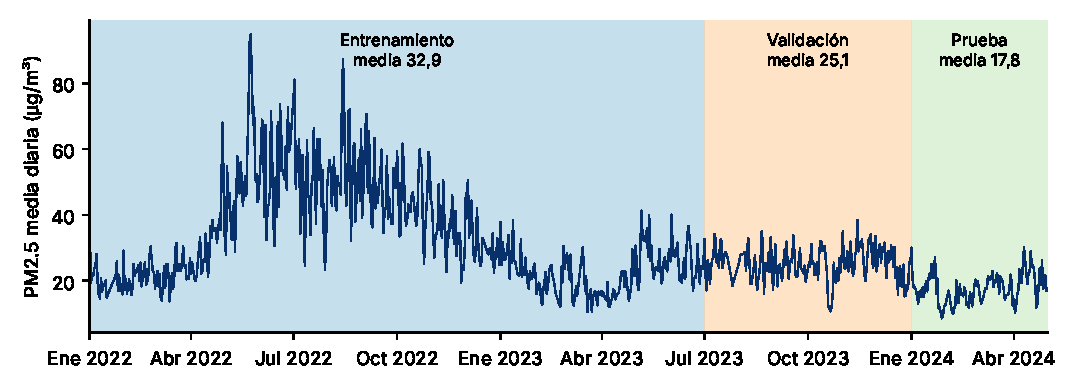
\includegraphics[width=\columnwidth]{figures/14_particiones_cronologicas.pdf}
\caption{Partición cronológica sobre la media diaria de PM2.5 (días con al menos 18 horas medidas). Se indica la media de la respuesta de cada bloque.}
\label{fig:part}
\end{figure}

\subsection{Preprocesamiento dentro del pipeline y prevención de fuga}

El escalado se ejecuta dentro de un \texttt{Pipeline} de scikit-learn: las nueve variables de historial se estandarizan con la media y la desviación del entrenamiento, y esos parámetros se aplican sin reajuste a validación y prueba. Ajustar el escalador con todos los datos filtraría información de los bloques posteriores: la media de $\mathrm{PM}_{2{,}5}(t)$ es de 32,94 en entrenamiento y de 28,98 en el conjunto completo.

La ausencia de fuga se comprueba de forma explícita con un guion reproducible (\texttt{scripts/02\_verificar\_fuga.py}) que ejecuta 12 verificaciones, todas superadas (Tabla~\ref{tab:fuga}). La prueba central altera por completo los valores posteriores a un instante de corte y comprueba que las entradas en ese instante no cambian. Como control negativo, se añade a propósito una variable con información futura y se confirma que la prueba la detecta.

\begin{table}[t]
\centering
\caption{Comprobaciones de ausencia de fuga de información.}
\label{tab:fuga}
\small
\begin{tabular}{@{}p{5.9cm}c@{}}
\toprule
Comprobación & Resultado \\
\midrule
Recálculo independiente con solo el pasado (500 filas) & Superada \\
Las entradas no cambian si se altera el futuro (8 cortes) & Superada \\
Respuesta igual a $\mathrm{PM}_{2{,}5}(t+1)$ y calendario de $t+1$ & Superada \\
Bloques ordenados, disjuntos y completos & Superada \\
Filas con hueco excluidas, sin ceros inventados & Superada \\
Escalador ajustado solo con entrenamiento (con y sin calendario) & Superada \\
Control negativo: una fuga deliberada es detectada & Superada \\
\bottomrule
\end{tabular}
\end{table}
